\documentclass[12pt, a4paper]{report}

% Packages :

\usepackage[french]{babel}
\usepackage[utf8]{inputenc}
\usepackage[T1]{fontenc}
\usepackage[pdftex, pdfauthor={Bacomathiques}]{hyperref}
\usepackage{sectsty}
\usepackage[explicit]{titlesec}
\usepackage{xcolor}
\usepackage{amsmath}
\usepackage{amssymb}
\usepackage{amsthm}
\usepackage{fourier}
\usepackage{titlesec}
\usepackage{fancyhdr}
\usepackage{catchfilebetweentags}
\usepackage[french, capitalise, noabbrev]{cleveref}
\usepackage[fit, breakall]{truncate}
\usepackage[margin=3cm]{geometry}
\usepackage{tocloft}
\usepackage{tikz}
\usepackage{tocloft}
\usepackage{microtype}
\usepackage{listings}
\usepackage{tabularx}
\usepackage{calc}
\usepackage[export]{adjustbox}
\usepackage[most]{tcolorbox}
\usepackage{standalone}
\usepackage{xlop}
\usepackage{etoolbox}
\usepackage{environ}

\usetikzlibrary{arrows.meta}
\usetikzlibrary{trees}

% Paramètres :

\author{Bacomathiques}
\definecolor{graphe}{HTML}{93c9ff}
\setcounter{MaxMatrixCols}{12}
\setlength{\parindent}{0pt}
\setlength{\fboxsep}{0pt}
%\pdfsuppresswarningpagegroup=1

% Code :

\lstdefinestyle{style}{
	backgroundcolor=\color{white},
	commentstyle=\em\color[HTML]{999988},
	keywordstyle=\bfseries,
	identifierstyle=\normalfont,
	stringstyle=\color[rgb]{0.87, 0.07, 0.27},
	basicstyle=\ttfamily\color{black},
	breakatwhitespace=false,
	breaklines=true,
	captionpos=b,
	keepspaces=true,
	numbers=left,
	numbersep=5pt,
	showspaces=false,
	showstringspaces=false,
	showtabs=false,
	tabsize=2,
	numbers=none
}

\lstset{style=style}
\lstset{
	literate=
	{á}{{\'a}}1
	{à}{{\`a}}1
	{ã}{{\~a}}1
	{é}{{\'e}}1
	{ê}{{\^e}}1
	{í}{{\'i}}1
	{ó}{{\'o}}1
	{õ}{{\~o}}1
	{ú}{{\'u}}1
	{ü}{{\"u}}1
	{ç}{{\c{c}}}1
}

\lstset{
	framextopmargin=10pt,
	framexrightmargin=10pt,
	framexbottommargin=10pt,
	framexleftmargin=10pt,
	xleftmargin=10pt,
	xrightmargin=10pt,
}

% Couleurs :

\definecolor{title}{HTML}{912c21}
\definecolor{section}{HTML}{1c567d}
\definecolor{subsection}{HTML}{2980b9}

\definecolor{rule}{HTML}{c4c4c4}

\definecolor{formula}{HTML}{ebf3fb}
\definecolor{formula-left}{HTML}{3583d6}

\definecolor{tip}{HTML}{dcf3d8}
\definecolor{tip-left}{HTML}{26a65b}

\definecolor{demonstration}{HTML}{fff8de}
\definecolor{demonstration-left}{HTML}{f1c40f}

\definecolor{exercise}{HTML}{e0f2f1}
\definecolor{exercise-left}{HTML}{009688}

\definecolor{correction}{HTML}{e0f7fa}
\definecolor{correction-left}{HTML}{00bcd4}

\definecolor{toc}{HTML}{fceae9}
\definecolor{toc-left}{HTML}{e74c3c}
\definecolor{toc-dark}{HTML}{87281f}

% Titres :

\renewcommand{\thesection}{\Roman{section} - }
\renewcommand{\thesubsection}{\arabic{subsection}. }

\newcommand{\sectionstyle}{\normalfont\LARGE\bfseries\color{section}}
\titleformat{\section}{\sectionstyle}{\thesection #1}{0pt}{}
\titleformat{name=\section, numberless}{\sectionstyle}{#1}{0pt}{}

\newcommand{\subsectionstyle}{\normalfont\Large\bfseries\color{subsection}}
\titleformat{\subsection}{\subsectionstyle}{\thesubsection #1}{0pt}{}
\titleformat{name=\subsection, numberless}{\subsectionstyle}{#1}{0pt}{}

\titlelabel{\thetitle\ }

% Table des matières :

\addto\captionsfrench{\renewcommand\contentsname{}}
\renewcommand{\cftsecpagefont}{\color{toc-dark}}
\renewcommand{\cftsubsecpagefont}{\color{toc-dark}}
\renewcommand{\cftsecleader}{\cftdotfill{\cftdotsep}}
\renewcommand{\cftsecfont}{\bfseries}
\renewcommand{\cftsecpagefont}{\bfseries\color{toc-dark}}
\setlength{\cftbeforetoctitleskip}{0pt}
\setlength{\cftaftertoctitleskip}{0pt}
\setlength{\cftsecindent}{0pt}
\setlength{\cftsubsecindent}{20pt}
\setlength{\cftsubsecnumwidth}{20pt}

% Commandes :

\newcommand{\newpar}{\\[\medskipamount]}
\newcommand{\lesson}[3]{%
	\newcommand{\level}{#1}%
	\newcommand{\id}{#2}%
	\hypersetup{pdftitle={#3}}
	\begin{center}%
		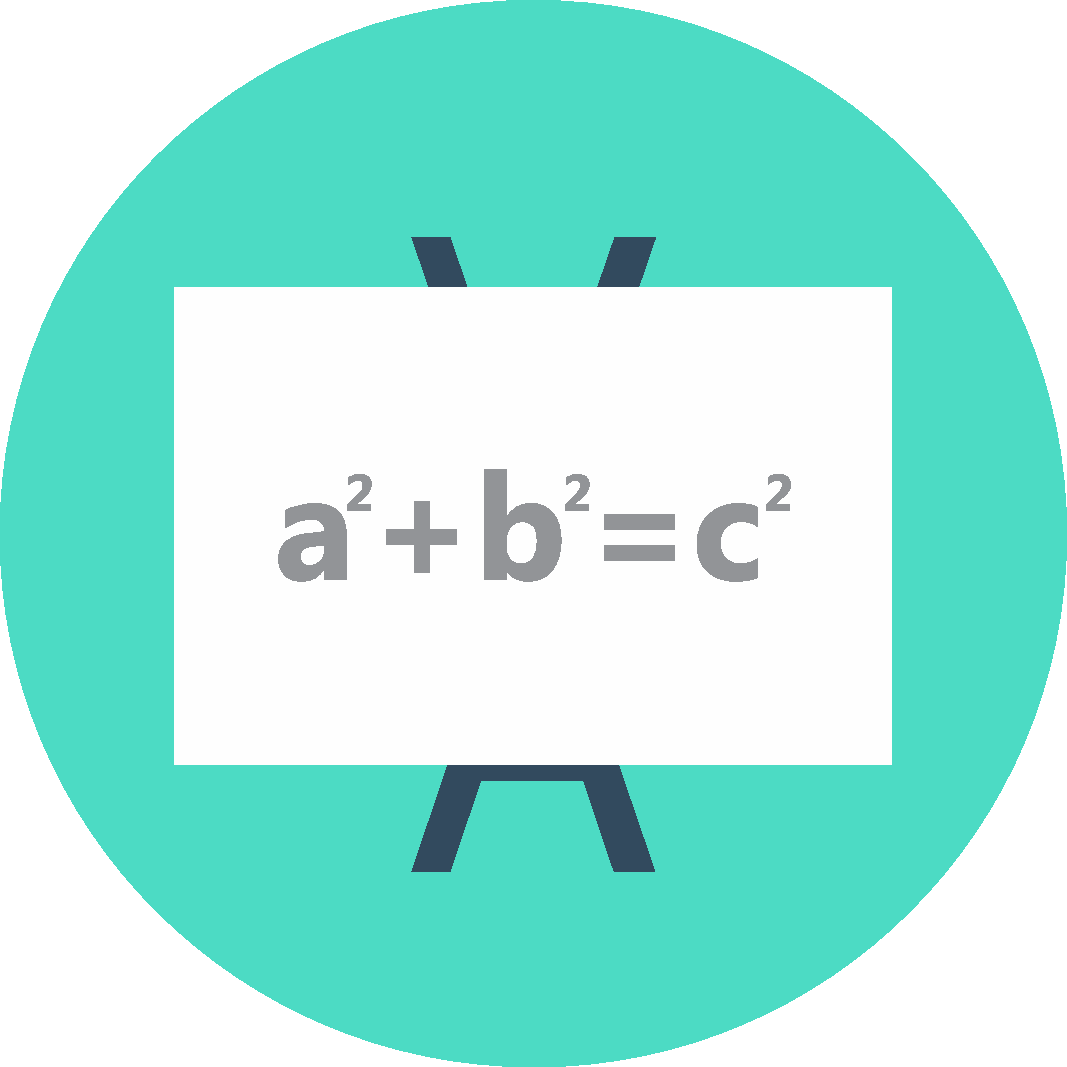
\includegraphics[width=150px]{\imagespath/bacomathiques}%
		
		\vspace{30pt}%
		{\Huge\color{title} #3}%
		
		\vspace{10pt}%
		{Bacomathiques --- \href{https://bacomathiqu.es/cours/#1/#2}{\color{section} https://bacomathiqu.es}}%
		
		\vspace{20pt}%
	\end{center}%
	\begin{toc}
		\tableofcontents%
	\end{toc}
	\thispagestyle{empty}%
	\newpage%
	\setcounter{page}{1}%
}
\newcommand{\imagespath}{../../images}
\newcommand{\lessonimagespath}{\imagespath/lessons/\level/\id/}
\newcommand{\includelatexpicture}[2][\textwidth - 100pt]{%
	\begin{center}%
		\resizebox{#1}{!}{%
			\input{\lessonimagespath#2}%
		}%
	\end{center}%
	\medskip%
}
\newcommand{\includeimage}[1]{%
	\begin{center}%
		\includegraphics{\lessonimagespath#1}%
	\end{center}%
	\medskip%
}
\newcommand{\includerepresentation}[1]{%
	\begin{center}%
		\setlength{\fboxrule}{0.5pt}%
		\href{https://www.geogebra.org/m/#1}{\includegraphics[width=\textwidth-1pt,fbox]{\lessonimagespath#1}}%
	\end{center}%
}
\newcommand{\floor}[1]{\lfloor #1 \rfloor}

\makeatletter
\newcommand\inputcontent{\@ifstar{\inputcontent@star}{\inputcontent@nostar}}
\newcommand{\inputcontent@star}[1]{%
	\ExecuteMetaData[#1]{content}%
}
\newcommand{\inputcontent@nostar}[1]{%
	\newpage%
	\inputcontent@star{#1}%
}
\makeatother

\let\oldsection\section
\renewcommand\section{\clearpage\oldsection}
\newcommand{\contentwidth}[1][medium]{}

% En-têtes :

\pagestyle{fancy}

\renewcommand{\sectionmark}[1]{\markboth{\thesection \ #1}{}}

\fancyhead[R]{\truncate{0.23\textwidth}{\color{title}\thepage}}
\fancyhead[L]{\truncate{0.73\textwidth}{\color{title}\leftmark}}
\fancyfoot[C]{\scriptsize \href{https://bacomathiqu.es/cours/\level/\id}{\texttt{bacomathiqu.es}}}

\makeatletter
\patchcmd{\f@nch@head}{\rlap}{\color{rule}\rlap}{}{}
\patchcmd{\headrule}{\hrule}{\color{rule}\hrule}{}{}
\makeatother

% Environnements :

\newenvironment{nosummary}{}{}
\newcommand{\tcolorboxtitle}[2]{\setlength{\fboxsep}{2.5pt}\hspace{-10pt}\colorbox{#1-left}{\hspace{8pt}\MakeUppercase{#2} \hspace{2pt} \includegraphics[height=0.8em]{\imagespath/bubbles/#1}\hspace{5pt}}}
\newcommand{\tcolorboxsubtitle}[2]{\ifstrempty{#2}{}{\textcolor{#1-left}{\large#2}\\[\medskipamount]}}
\tcbset{
	frame hidden,
	boxrule=0pt,
	boxsep=0pt,
	enlarge bottom by=8.5pt,
	enhanced jigsaw,
	boxed title style={sharp corners,boxrule=0pt,coltitle={white},titlerule=0pt},
	fonttitle=\fontsize{6pt}{6pt}\bfseries\boldmath,
	top=10pt,
	right=10pt,
	bottom=10pt,
	left=10pt,
	arc=0pt,
	outer arc=0pt,
}
\newtcolorbox{toc}[1][]{
	colback=toc,
	borderline west={3pt}{0pt}{toc-left},
	title=\tcolorboxtitle{toc}{Table des matières},
	colbacktitle=toc,
	before upper={\tcolorboxsubtitle{toc}{#1}}
}
\newtcolorbox{formula}[1][]{
	colback=formula,
	borderline west={3pt}{0pt}{formula-left},
	title=\tcolorboxtitle{formula}{À retenir},
	colbacktitle=formula,
	before upper={\tcolorboxsubtitle{formula}{#1}}
}
\newtcolorbox{tip}[1][]{
	colback=tip,
	borderline west={3pt}{0pt}{tip-left},
	title=\tcolorboxtitle{tip}{À lire},
	colbacktitle=tip,
	before upper={\tcolorboxsubtitle{tip}{#1}}
}
\newtcolorbox{demonstration}[1][]{
	colback=demonstration,
	borderline west={3pt}{0pt}{demonstration-left},
	title=\tcolorboxtitle{demonstration}{Démonstration},
	colbacktitle=demonstration,
	before upper={\tcolorboxsubtitle{demonstration}{#1}}
}

\NewEnviron{whitetabularx}[1]{%
	\renewcommand{\arraystretch}{2.5}
	\colorbox{white}{%
		\begin{tabularx}{\textwidth}{#1}%
			\BODY%
		\end{tabularx}%
	}%
}

% Longueurs :

\newlength{\espacetitreliste}
\setlength{\espacetitreliste}{-16pt}
\newcommand{\entretitreetliste}{\vspace{\espacetitreliste}}

\begin{document}
	%<*content>
	\lesson{terminale}{9}{denombrement}{Dénombrement}

	\header{caption}{On peut utiliser le dénombrement pour connaître le nombre de combinaisons
		possibles dans un jeu de cartes.}

	\header{excerpt}{En mathématiques, le dénombrement est la détermination du nombre d'éléments
		d'un ensemble. Nous allons voir, dans ce chapitre, toutes les formules utiles
		au dénombrement (combinaisons, permutations, nombre de sous-ensembles, principe
		additif et multiplicatif, etc...). Nous ferons également quelques rappels concernant
		la théorie des ensembles.}

	\header{difficulty}{2}

	\section{Définitions}

	\subsection{Ensemble d'éléments}

	Cette partie donne quelques rappels sur la notion d'ensemble en mathématiques.

	\begin{formula}[Définition]
		Un \textbf{ensemble} $E$ désigne une collection finie ou infinie d'objets distincts qu'on appelle ses \textbf{éléments}.
		\newpar
		On note $x \in E$ si l'objet $x$ appartient à $E$. Dans le cas contraire, on note $x \notin E$.
	\end{formula}

	À noter que l'ordre des objets n'a aucune importance lorsque l'on compare deux ensembles.

	\begin{tip}[Exemple]
		Voici quelques exemples d'ensembles :
		\begin{itemize}
			\item $\{2; 4; 6\}$ est un ensemble contenant $3$ éléments.
			\item $\mathbb{Z}$ et $\mathbb{R}$ sont deux ensembles contenant une infinité d'éléments.
			\item $\{\}$ est un ensemble ne contenant aucun élément : c'est \textbf{l'ensemble vide}, noté $\emptyset$.
			\item $\{1\}$ est un ensemble content $1$ élément : c'est un \textbf{singleton}.
		\end{itemize}
	\end{tip}

	\begin{tip}
		Il est possible de créer des ensembles contenant autre choses que des nombres. Par exemple, on définit les fonctions $f : x \mapsto x^2$ et $g : x \mapsto x^3 + 1$. Alors l'ensemble $E = \{f; g\}$ est un ensemble contenant des fonctions.
	\end{tip}

	\begin{formula}[Réunion et intersection]
		Soient $E$ et $F$ deux ensembles.
		\begin{itemize}
			\item Leur \textbf{réunion} notée $E \, \cup \, F$ est l'ensemble constitué des éléments de $E$ et des éléments de $F$.
			\item Leur \textbf{intersection} notée $E \, \cap \, F$ est l'ensemble constitué des éléments communs à $E$ et $F$.
			\item Si $E \, \cap \, F = \emptyset$, on dit que $E$ et $F$ sont \textbf{disjoints}.
		\end{itemize}
	\end{formula}

	\subsection{Sous-ensemble}

	\begin{formula}[Définition]
		Soient $E$ et $F$ deux ensembles. On dit que $F$ est un \textbf{sous-ensemble} (ou une partie) de $E$ si tout élément de $F$ est un élément de $E$.
		\newpar
		On note ceci par $F \subset E$ (qui signifie ``$F$ est inclus dans $E$'').
	\end{formula}


	\begin{tip}[Exemple]
		Soient $E$ et $F$ deux ensembles. Alors $E \, \cap \, F \subset E$ et $E \, \cap \, F \subset F$.
	\end{tip}

	\subsection{Liste d'éléments}

	Nous allons désormais voir un type de collection similaire aux ensembles, mais qui prend en compte l'ordre des éléments.

	\begin{formula}[Définition]
		Un \textbf{$p$-uplet} (ou une $p$-liste) d'un ensemble $E$ désigne une collection ordonnée de $p$ éléments de $E$.
	\end{formula}

	Remarquons que l'on ne demande pas que les éléments d'un $p$-uplet soient tous distincts.

	\begin{tip}[Attention à l'ordre des éléments]
		Il faut bien faire attention à l'ordre des éléments ! Prenons par exemple deux points du plan $A = (1; 2)$ et $B = (2; 1)$.
		\newpar
		On peut voir $A$ et $B$ comme des $2$-uplets de $\mathbb{R}$. Or, ce sont deux points différents, d'où la nécessité de bien faire attention à ne pas mélanger $(1; 2)$ et $(2; 1)$.
	\end{tip}

	\begin{tip}[Notation]
		Bien que l'on note un ensemble avec des accolades, on note plutôt un $p$-uplet avec des parenthèses. Ainsi :
		\begin{itemize}
			\item $\{1; 2; 3; 4; 5\}$ désigne l'ensemble constitué des nombres entiers de $1$ à $5$ (on a $\{1; 2; 3; 4; 5\} = \{2; 1; 3; 4; 5\} = \{5; 4; 3; 2; 1\} = ...$).
			\item $(1; 2; 3; 4; 5)$ désigne le $5$-uplet constitué des nombres entiers de $1$ à $5$ (on a $(1; 2; 3; 4; 5) \neq (2; 1; 3; 4; 5) \neq (5; 4; 3; 2; 1) \neq ...$).
		\end{itemize}
	\end{tip}

	\section{Combinaisons}

	\subsection{Factorielle}

	\begin{formula}[Définition]
		Soit $n$ un nombre entier. On appelle factorielle de $n$ le nombre entier suivant :
		\[ n! = 1 \times 2 \times \dots \times n \]
	\end{formula}

	\begin{tip}[Convention]
		Par convention, on pose $0! = 1$.
	\end{tip}

	Il est très courant de rencontrer des calculs avec des factorielles en mathématiques, leur utilisation ne se limitant pas au dénombrement.

	\subsection{Définition}

	\begin{formula}[Définition]
		Une \textbf{combinaison} de $k$ éléments parmi $n$ éléments, notée $\binom{n}{k}$, est le nombre de sous-ensembles de $k$ éléments que possède un ensemble de $n$ éléments.
	\end{formula}

	\begin{formula}[Calcul d'une combinaison]
		Soient $n$ et $k$ deux entiers. Alors $\binom{n}{k} = \frac{n!}{(n-k)!k!}$.
	\end{formula}

	\begin{tip}[Exemple]
		Soit $E = \{1, 2, 3, \dots, 30 \}$. On cherche à connaître le nombre de sous-ensembles de $3$ éléments que possède $E$. Pour cela, il suffit d'appliquer la formule :
		\[ \binom{30}{3} = \frac{30!}{27!3!} = \frac{28 \times 29 \times 30}{1 \times 2 \times 3} = 4060 \]
		$E$ contient $4060$ sous-ensembles de $3$ éléments.
	\end{tip}

	\subsection{Formules}

	\begin{formula}[Formules]
		Soient $n$ et $k$ deux entiers.
		\begin{itemize}
			\item $\binom{n}{0} = \binom{n}{n} = 1$
			\item $\binom{n}{1} = \binom{n}{n-1} = n$
			\item $\binom{n}{k} = \binom{n}{n-k}$
		\end{itemize}
	\end{formula}

	\begin{tip}[Triangle de Pascal]
		Une autre formule très utile est $\binom{n}{k} + \binom{n}{k+1} = \binom{n+1}{k+1}$. Elle peut se retrouver à l'aide du triangle de Pascal, que l'on construit comme tel :
		\begin{enumerate}
			\item Dans une pyramide, on place un $1$ au sommet de la pyramide.
			\item On place $1$ et $1$ en dessous, de part et d'autre.
			\item Les extrémités des lignes sont toujours des $1$, et les autres nombres sont la somme des deux nombres directement au-dessus.
		\end{enumerate}
		Les premières lignes du triangle de Pascal sont donc :
		\includelatexpicture[100pt]{pascal}

		Ainsi, le $k$-ième coefficient de la $n$-ième ligne est égal à $\binom{n}{k}$ (en partant de $0$).
	\end{tip}

	\section{Dénombrement}

	\subsection{Principe additif}

	\begin{formula}[Principe additif]
		Soient $E$ et $F$ deux ensembles disjoints contenant respectivement $n$ et $m$ éléments. Alors $E \, \cup \, F$ contient $n + m$ éléments.
	\end{formula}

	\begin{tip}[Exemple]
		Si on pose $E = \{1; 3; 5\}$ et $F = \{2; 4; 6; 8\}$. $E$ et $F$ sont alors bien disjoints, donc $E \, \cup \, F$ contient $3 + 4 = 7$ éléments.
	\end{tip}

	\subsection{Principe multiplicatif}

	Commençons cette sous-section par une définition.

	\begin{formula}[Produit cartésien]
		Soient $E$ et $F$ deux ensembles. Leur produit cartésien $E \times F$ est l'ensemble des couples $(e; f)$ où $e \in E$ et $f \in F$.
	\end{formula}

	\begin{tip}[Exemple]
		Cette définition peut sembler un peu compliquée, mais elle est en faite très intuitive. Prenons $E = \{1; 2; 3\}$ et $F = \{4; 5\}$.
		\newpar
		Alors on a $E \times F = \{(1; 4); (1; 5); (2; 4); (2; 5); (3; 4); (3; 5)\}$.
	\end{tip}

	\begin{tip}[Construction du plan cartésien]
		Prenons maintenant $E = F = \mathbb{R}$. Le produit cartésien $E \times F$ est l'ensemble des couples $(x; y)$ où $x \in \mathbb{R}$ et $y \in \mathbb{R}$.
		\newpar
		Il s'agit en fait du plan cartésien.
	\end{tip}

	\begin{formula}[Principe multiplicatif]
		Soient $E$ et $F$ deux ensembles contenant respectivement $n$ et $m$ éléments. Alors $E \times F$ contient $n \times m$ éléments.
	\end{formula}

	Ce principe (tout comme le principe additif vu précédemment) sont notamment utilisés en probabilités.

	\subsection{Formules de dénombrement}

	\begin{formula}[Permutations]
		Soit $E$ un ensemble de taille $n$. On appelle \textbf{permutation} de $E$ tout $n$-uplet d'éléments distincts de $E$.
	\end{formula}

	\begin{tip}[Exemple]
		Prenons $E = \{1; 2; 3\}$. Alors $E$ admet $6$ permutations qui sont :
		\begin{itemize}
			\item $(1; 2; 3)$
			\item $(1; 3; 2)$
			\item $(2; 1; 3)$
			\item $(2; 3; 1)$
			\item $(3; 1; 2)$
			\item $(3; 2; 1)$
		\end{itemize}
	\end{tip}

	\begin{formula}[Formules]
		Soit $E$ un ensemble possédant $n$ éléments.
		\begin{itemize}
			\item Le nombre de $p$-uplets d'éléments de $E$ est égal à $n^p$.
			\item Le nombre de $p$-uplets d'éléments distincts de $E$ est égal à $\frac{n!}{(n-p)!}$.
			\item Le nombre de permutations de $E$ est égal à $n!$.
			\item Le nombre de sous-ensembles de $E$ est égal à $2^n$.
			\item Le nombre de sous-ensembles de $k$ éléments que possède $E$ est égal à $\binom{n}{k}$ (pour rappel).
		\end{itemize}
	\end{formula}

	\begin{nosummary}
		À noter également une dernière petite formule qu'il peut être utile de savoir démontrer à l'aide des formules ci-dessus.

		\begin{formula}
			Pour tout $n \in \mathbb{N}$ :
			\[ \sum_{k = 0}^n \binom{n}{k} = 2^n \]
		\end{formula}

		\begin{demonstration}
			Soit $n \in \mathbb{N}$ et soit $E$ un ensemble à $n$ éléments.
			\newpar
			Par la dernière formule de dénombrement, $E$ a $\binom{n}{0}$ sous-ensembles qui possèdent $0$ éléments, $\binom{n}{1}$ sous-ensembles qui possèdent $1$ éléments, ...
			\newpar
			En fait, pour tout $k$ compris entre $0$ et $n$, $E$ a exactement $\binom{n}{k}$ sous-ensembles qui possèdent $k$ éléments (toujours d'après la dernière formule).
			\newpar
			Donc finalement, on obtient bien que la somme des $\binom{n}{k}$ vaut $2^n$ (qui est, d'après l'avant-dernière formule, le nombre de sous-ensembles que possède $E$).
		\end{demonstration}
	\end{nosummary}
	%</content>
\end{document}
